\section{ROS file system}

The foundation of the ROS file system revolves around packages, depicted in the diagram below. 
\begin{figure}[H]
    \centering
    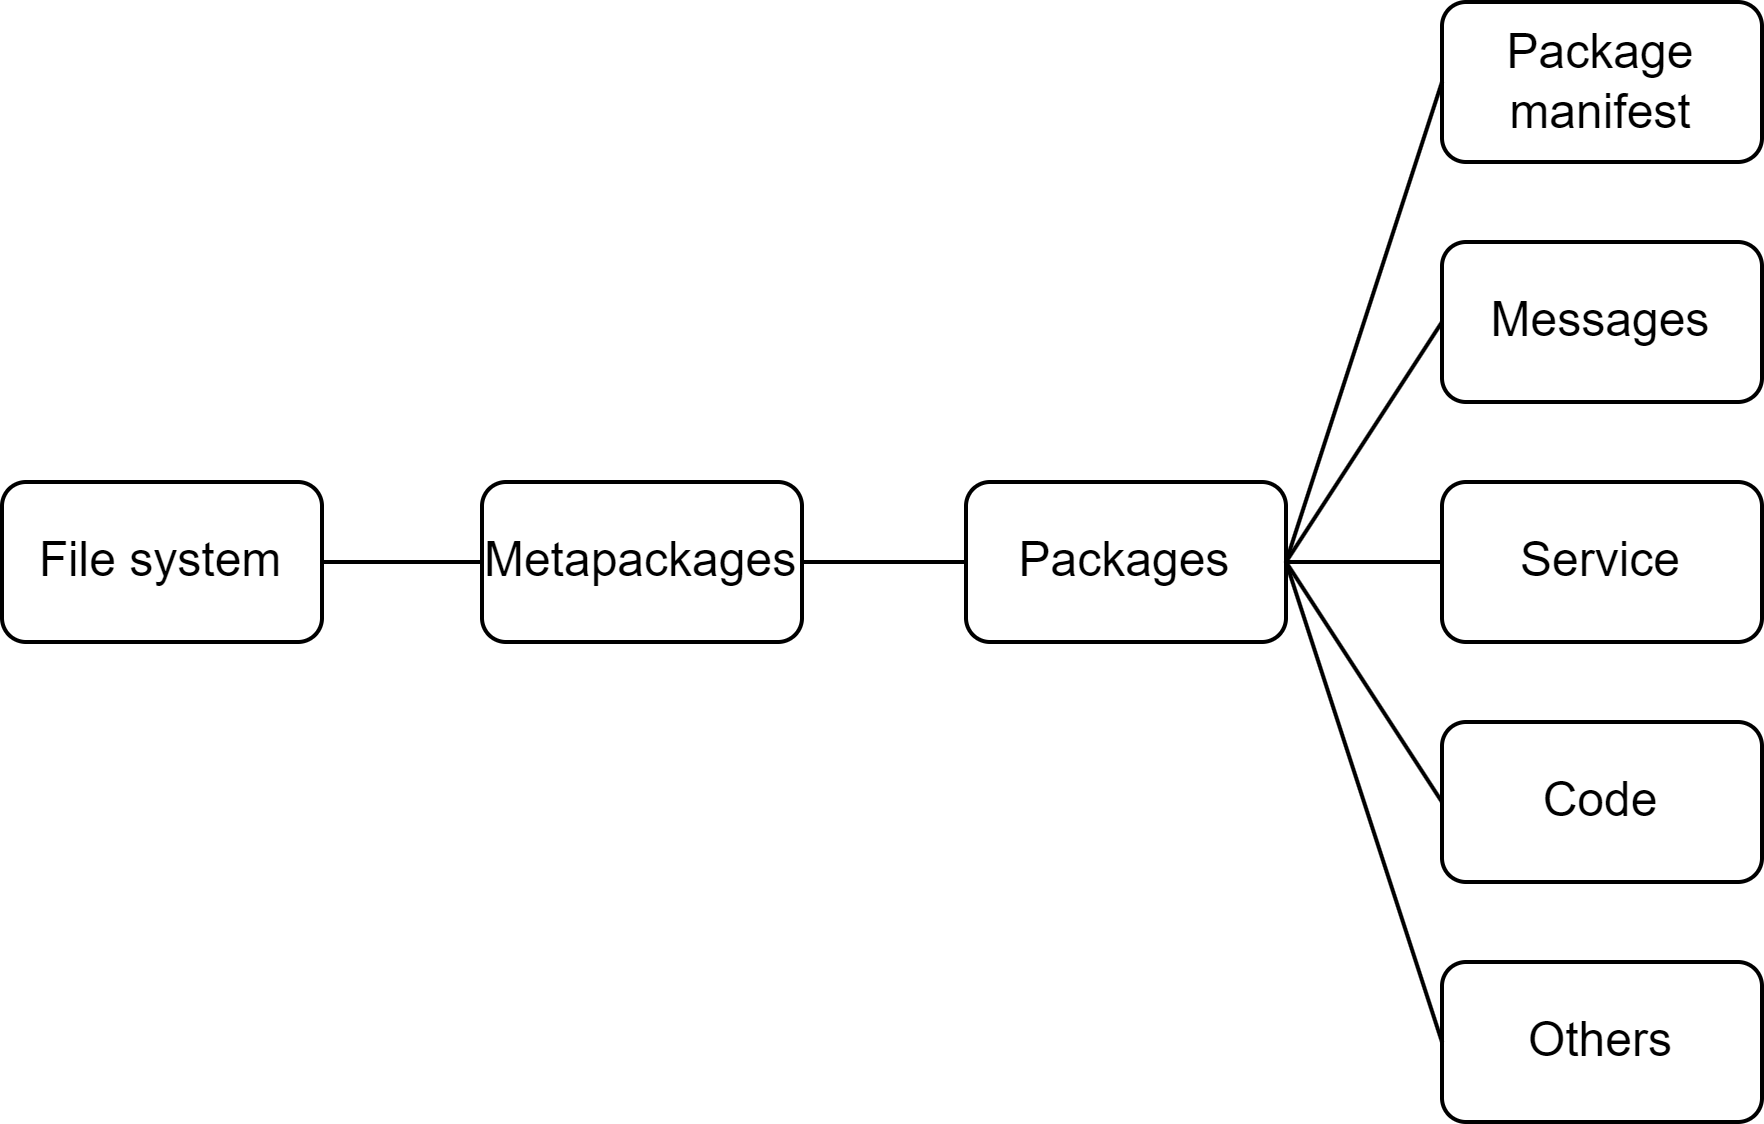
\includegraphics[width=0.75\linewidth]{images/fs.png}
    \caption{ROS file system}
\end{figure}
Packages serve as the fundamental units within the ROS file system. 
They are essential references for most ROS commands and encompass nodes, messages, and services. 
Each package is described by a \texttt{package.xml} file and acts as a mandatory container for its contents.

Additionally, there are metapackages, which aggregate logically related elements. 
Unlike packages, metapackages are not directly utilized when navigating the ROS file system. 
They contain other packages and are described by a package.xml file as well, but they are not obligatory components.

\subsection{Packages}
Packages serve as fundamental units within the ROS file system, acting as the cornerstone for most ROS commands. 
They encapsulate nodes, messages, and services, providing a structured organization for ROS functionalities.
Each package is described by a package.xml file, serving as a mandatory container that delineates the package's properties and dependencies.
The general structure of a package includes the following components:
\begin{itemize}
    \item Folder Structure:
        \begin{itemize}
            \item /src, /include, /scripts (for coding).
            \item /launch (for launch files).
            \item /config (for configuration files).
        \end{itemize}
    \item Required Files:
        \begin{itemize}
            \item CMakeLists.txt: contains build rules for catkin.
            \item package.xml: provides metadata for ROS.\@
        \end{itemize}
\end{itemize}

\subsection{Metapackages}
Metapackages are collections of logically related elements within ROS, serving as aggregations rather than individual components. 
Unlike regular packages, they are not typically used when navigating the ROS file system. 
Metapackages encompass other packages and are described by a package.xml file, yet they are not obligatory structures within ROS.\@